% 第 3 题四图像：按固定源 PDF 矢量路径换算（1 pt → 0.03515 cm）。
% 原点取 (A) 面板原点（源页 (150.89, 350.45) pt），y 向上；1 单位 = 25.5 pt（横纵同比例）。
% 四面板原点（相对本坐标系）：(A)(0,0)、(B)(169.57,0)、(C)(−0.30,−93.30)、(D)(170.16,−93.30)。
% 每面板：y 轴自原点下 38.25 上至箭头尖点 38.25；x 轴左 63.76 右至箭头尖点 63.76；
% y 轴刻度线 (0,25.5)–(3.06,25.5) 标「1」；x 轴刻度线在 ±40.06（=π/2×25.5）各长 3.06。
% 曲线线宽 0.8pt（源为轴 0.398 的 2 倍）；四曲线形状经矢量采样数值拟合为
% (A) sign(x)·sin²x、(B) |sin x|、(C) sign(x)·sin(x²)、(D) sin(x²)
% （源内四图无函数式标注，拟合残差 ≤0.003 单位；照此绘制，不写入题面）。
% 轴标签 y/x/O、刻度「1」与分式「−π/2」「π/2」按源字形框中心显式定位；
% (C) 面板左标签整组位于 x 轴上方（源内如此，照录）；选项标号 (A)(B)(C)(D) 在各面板下方源位。
% 【修复轮修正】初版按字框中心定位使「−π/2」「π/2」的 π 与 x 轴线墨迹相融（试题版 P1
% figure_label 600 dpi 连通域查出：π 腿跨轴、与轴同属一分量）。按源墨迹实测重定位：
% 源内轴下标签的 π 顶横距轴心 3.7 pt（600 dpi 行测 31 px/8.333），2 底距轴 ≥2.2 pt——
% 七个轴下标签整体下移 4.86 pt、C 面板轴上标签上移 2.0 pt（其余水平位置不变）。
\begin{tikzpicture}[line cap=round,line join=round,font=\small,x=0.03515cm,y=0.03515cm]
% ===== 面板 (A) =====
\draw[->] (0,-38.25)--(0,38.25);
\draw[->] (-63.76,0)--(63.76,0);
\draw (0,25.5)--(3.06,25.5);
\draw (-40.06,0)--(-40.06,3.06);
\draw (40.06,0)--(40.06,3.06);
\draw[line width=0.8pt] plot[domain=-2:2,samples=201] ({25.5*\x},{25.5*sign(\x)*sin(deg(\x))*sin(deg(\x))});
\node[anchor=center,inner sep=0] at (-6.59,39.62) {\(y\)};
\node[anchor=center,inner sep=0] at (6.38,24.72) {\(1\)};
\node[anchor=center,inner sep=0] at (-7.94,-8.28) {\(O\)};
\node[anchor=center,inner sep=0] at (63.83,-5.63) {\(x\)};
\node[anchor=center,inner sep=0] at (-40.64,-13.23) {\(-\dfrac{\pi}{2}\)};
\node[anchor=center,inner sep=0] at (40.00,-13.73) {\(\dfrac{\pi}{2}\)};
% ===== 面板 (B)（右移 169.57）=====
\begin{scope}[shift={(169.57,0)}]
\draw[->] (0,-38.25)--(0,38.25);
\draw[->] (-63.76,0)--(63.76,0);
\draw (0,25.5)--(3.06,25.5);
\draw (-40.06,0)--(-40.06,3.06);
\draw (40.06,0)--(40.06,3.06);
\draw[line width=0.8pt] plot[domain=-2:2,samples=201] ({25.5*\x},{25.5*abs(sin(deg(\x)))});
\node[anchor=center,inner sep=0] at (-6.53,39.62) {\(y\)};
\node[anchor=center,inner sep=0] at (6.45,24.72) {\(1\)};
\node[anchor=center,inner sep=0] at (-7.88,-8.28) {\(O\)};
\node[anchor=center,inner sep=0] at (63.90,-5.63) {\(x\)};
\node[anchor=center,inner sep=0] at (-40.67,-13.23) {\(-\dfrac{\pi}{2}\)};
\node[anchor=center,inner sep=0] at (40.07,-13.73) {\(\dfrac{\pi}{2}\)};
\end{scope}
% ===== 面板 (C)（下移 93.30，左移 0.30）=====
\begin{scope}[shift={(-0.30,-93.30)}]
\draw[->] (0,-38.25)--(0,38.25);
\draw[->] (-63.76,0)--(63.76,0);
\draw (0,25.5)--(3.06,25.5);
\draw (-40.06,0)--(-40.06,3.06);
\draw (40.06,0)--(40.06,3.06);
\draw[line width=0.8pt] plot[domain=-2:2,samples=201] ({25.5*\x},{25.5*sign(\x)*sin(deg(\x*\x))});
\node[anchor=center,inner sep=0] at (-6.59,39.59) {\(y\)};
\node[anchor=center,inner sep=0] at (6.39,24.69) {\(1\)};
\node[anchor=center,inner sep=0] at (-7.94,-8.31) {\(O\)};
\node[anchor=center,inner sep=0] at (63.84,-5.66) {\(x\)};
\node[anchor=center,inner sep=0] at (-40.63,11.75) {\(-\dfrac{\pi}{2}\)};
\node[anchor=center,inner sep=0] at (40.01,-13.76) {\(\dfrac{\pi}{2}\)};
\end{scope}
% ===== 面板 (D)（下移 93.30，右移 170.16）=====
\begin{scope}[shift={(170.16,-93.30)}]
\draw[->] (0,-38.25)--(0,38.25);
\draw[->] (-63.76,0)--(63.76,0);
\draw (0,25.5)--(3.06,25.5);
\draw (-40.06,0)--(-40.06,3.06);
\draw (40.06,0)--(40.06,3.06);
\draw[line width=0.8pt] plot[domain=-2:2,samples=201] ({25.5*\x},{25.5*sin(deg(\x*\x))});
\node[anchor=center,inner sep=0] at (-6.53,39.59) {\(y\)};
\node[anchor=center,inner sep=0] at (6.45,24.69) {\(1\)};
\node[anchor=center,inner sep=0] at (-7.88,-8.31) {\(O\)};
\node[anchor=center,inner sep=0] at (63.90,-5.66) {\(x\)};
\node[anchor=center,inner sep=0] at (-40.60,-13.26) {\(-\dfrac{\pi}{2}\)};
\node[anchor=center,inner sep=0] at (40.07,-13.76) {\(\dfrac{\pi}{2}\)};
\end{scope}
% ===== 选项标号（照源字形框中心；置于各面板下方）=====
\node[anchor=center,inner sep=0] at (-75.44,-35.28) {(A)};
\node[anchor=center,inner sep=0] at (94.42,-35.28) {(B)};
\node[anchor=center,inner sep=0] at (-75.58,-128.62) {(C)};
\node[anchor=center,inner sep=0] at (94.71,-128.62) {(D)};
\end{tikzpicture}
